For the sample input:
\begin{verbatim}
4
2 1
3 3
4 4
5 2
\end{verbatim}

a possible valid output is:

\begin{verbatim}
6
2 0
2 3
5 3
5 2
4 2
4 4
\end{verbatim}

\begin{center}
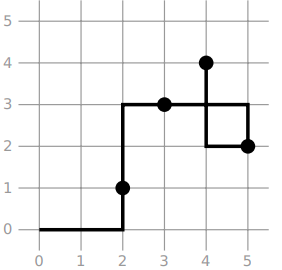
\includegraphics[scale=0.5]{1.png}
\end{center}

Please note this example is not among the actual inputs of this task.


\textbf{Visualizer}

In the attachments of this task, there is a script that allows you to visualize input and output files.

To visualize an input file, use the following command:

\texttt{python vis.py [input file]}

You can also visualize your solution for some input, using the following command.
Due to technical limitations, the provided visualizer shows only \texttt{the first $1000$ segments} of the output file.

\texttt{python vis.py [input file] --solution [output file]}

Example:

\texttt{python vis.py examples/00.in --solution examples/00.out}
